\documentclass[12pt]{article}
            \usepackage{sbc-template}
            \makeatletter
            \renewcommand{\inst}[1]{}
            \makeatother
            \usepackage{graphicx,url}
            \usepackage[utf8]{inputenc}
            \usepackage[T1]{fontenc}
            \usepackage[brazil]{babel}
            \usepackage{longtable,booktabs,array,tabularx}
            \usepackage{amsmath,amssymb}
            \usepackage{fvextra}
            \newcolumntype{Y}{>{\raggedright\arraybackslash}X}
            \newcolumntype{C}{>{\centering\arraybackslash}X}
            \setlength{\LTleft}{0pt}
            \setlength{\LTright}{0pt}
            \RecustomVerbatimEnvironment{verbatim}{Verbatim}{%
              breaklines=true,
              breakanywhere=true,
              breaksymbolleft={},
              fontsize=\small
            }
            \providecommand{\tightlist}{%%
              \setlength{\itemsep}{0pt}\setlength{\parskip}{0pt}}
            \providecommand{\pandocbounded}[1]{#1}
            \usepackage{fancyhdr}
            \pagestyle{fancy}
            \fancyhf{}
            \fancyfoot[R]{\thepage}
            \fancyfoot[L]{SANTOS, Anderson F. P. dos — Fundamentos de Reservoir Computing}
            \renewcommand{\headrulewidth}{0pt}
            \renewcommand{\footrulewidth}{0.4pt}
            \sloppy
            \title{Fundamentos de Reservoir Computing}
            \author{Anderson Fernandes Pereira dos Santos}
            \address{Instituto Militar de Engenharia (IME), Rio de Janeiro, Brazil \\
Venturus Innovation Center, Campinas, Brazil \\
\texttt{anderson@ime.eb.br} | \texttt{anderson.santos@venturus.org.br}}
            \begin{document}

            \maketitle

            \begin{resumo}
            Este artigo apresenta Reservoir Computing (RC) como o primeiro grande degrau teórico da série. O foco não é apenas definir o termo, mas mostrar como um reservatório transforma uma sequência em uma representação dinâmica heterogenea, não linear e com memória distribuída. Além da intuição e das equações, o texto introduz uma camada que faltava na versão anterior: como avaliar o que o RC realmente entrega em três níveis diferentes: qualidade da representação interna, qualidade da previsão final e qualidade da estabilidade experimental. No recorte Favorita, o RC clássico funciona, produz estados coerentes e previsões reprodutíveis, mas a configuração default ainda fica atrás de \texttt{Seasonal\ Naive} e \texttt{ETS}. Também mostramos que seed, \texttt{spectral\_radius}, \texttt{leak\_rate}, \texttt{washout} e \texttt{n\_reservoir} mudam materialmente o erro, o que transforma esses hiperparâmetros em decisões de projeto, e não em detalhes cosméticos.
            \end{resumo}

            \section{O que o leitor vai aprender}\label{1-o-que-o-leitor-vai-aprender}

Ao final deste artigo, você será capaz de:

\begin{enumerate}
\def\labelenumi{\arabic{enumi}.}
\tightlist
\item
  definir um reservatório clássico de forma matemática;
\item
  distinguir estado interno, vetor de entrada e readout;
\item
  explicar o papel de \texttt{spectral\_radius}, \texttt{leak\_rate} e \texttt{washout};
\item
  mapear as equações de RC para a implementação em \texttt{code/rc/model.py};
\item
  separar qualidade da representação interna, qualidade da previsão final e qualidade da estabilidade experimental.
\end{enumerate}

\section{A intuição: o que um reservatório faz, antes da equação}\label{2-a-intuiuxe7uxe3o-o-que-um-reservatuxf3rio-faz-antes-da-equauxe7uxe3o}

Em um modelo tabular tradicional, as features costumam ser calculadas explicitamente: lags, médias móveis, indicadores de calendário e assim por diante. Em RC, a ideia é diferente. Em vez de escrever manualmente toda a representação temporal, injetamos a sequência em um sistema dinamico recorrente e usamos seus estados internos como uma base de representação.

A melhor imagem mental para um iniciante é esta:

\begin{itemize}
\tightlist
\item
  a entrada \(u_t\) entra no sistema no instante atual;
\item
  o sistema ainda guarda parte do que aconteceu antes;
\item
  essa mistura entre presente e passado gera um novo estado interno;
\item
  a previsão final e feita a partir desse estado.
\end{itemize}

Em outras palavras, o reservatório não tenta prever diretamente. Primeiro ele \textbf{transforma a sequência em estados internos}. Só depois o readout aprende a ler esses estados.

Se quisermos resumir RC em uma frase curta, ela seria:

\begin{quote}
o reservatório e um mecanismo fixo que converte sequências em representações dinâmicas; o readout e a parte treinada que converte essas representações em previsão.
\end{quote}

Essa divisão é importante porque reduz a carga conceitual:

\begin{enumerate}
\def\labelenumi{\arabic{enumi}.}
\tightlist
\item
  primeiro entendemos como o estado interno evolui;
\item
  depois entendemos como a previsão sai desse estado.
\end{enumerate}

\section{Construindo o modelo mínimo de RC}\label{3-construindo-o-modelo-muxednimo-de-rc}

Em muitos textos de RC, a equação do reservatório aparece pronta, em uma única linha. Para quem esta vendo o tema pela primeira vez, isso costuma ser brusco demais. Aqui vamos fazer o caminho inverso: começamos com a pergunta intuitiva, descemos até um único passo de atualizacao, olhamos um exemplo de uma única unidade e só entao escrevemos a equação completa.

\subsection{A pergunta central em um único passo}\label{31-a-pergunta-central-em-um-uxfanico-passo}

Em cada instante \(t\), o reservatório recebe uma entrada \(u_t\) e mantem internamente um estado \(x_{t-1}\) vindo do passo anterior. O problema do passo atual pode ser formulado assim:

\begin{quote}
dado o que entrou agora e dado o que o sistema ainda guarda do passado, como produzir o novo estado \(x_t\)?
\end{quote}

Essa pergunta já organiza quase todo o raciocinio. O novo estado precisa depender de duas coisas:

\begin{itemize}
\tightlist
\item
  da entrada atual;
\item
  da memória que o proprio sistema traz do passo anterior.
\end{itemize}

\subsection{Os ingredientes da atualizacao}\label{32-os-ingredientes-da-atualizacao}

Para responder a essa pergunta, o modelo usa:

\begin{itemize}
\tightlist
\item
  \(u_t \in \mathbb{R}^d\), o vetor de entrada no tempo \(t\);
\item
  \(x_{t-1} \in \mathbb{R}^N\), o estado interno do passo anterior;
\item
  \(W_{in}\), a matriz que projeta a entrada para o espaco do reservatório;
\item
  \(W_{res}\), a matriz recorrente interna, que mistura os componentes do proprio estado;
\item
  \(b\), um vetor de bias;
\item
  \(\alpha \in (0,1]\), o \texttt{leak\_rate}, que controlara quanto do estado novo realmente entra.
\end{itemize}

O ponto principal aqui não é decorar a notação. O ponto principal e perceber o papel de cada termo:

\begin{itemize}
\tightlist
\item
  \(W_{in} u_t\) traz o \textbf{efeito da entrada atual};
\item
  \(W_{res} x_{t-1}\) traz o \textbf{efeito do passado interno};
\item
  \(b\) apenas desloca essa resposta;
\item
  \(\alpha\) vai decidir quanto do estado novo substitui o antigo.
\end{itemize}

\subsection{Primeiro passo: montar a resposta bruta do sistema}\label{33-primeiro-passo-montar-a-resposta-bruta-do-sistema}

Antes de falar em "estado candidato", vale pensar no que acontece imediatamente quando somamos os efeitos do presente e do passado. Chamaremos essa soma de pre-ativacao:

\[
z_t = W_{res} x_{t-1} + W_{in} u_t + b.
\]

Essa expressão pode ser lida em voz alta assim:

\begin{quote}
resposta bruta no tempo \(t\) = efeito da memória anterior + efeito da entrada atual + bias.
\end{quote}

O vetor \(z_t\) ainda não é o novo estado final. Ele e apenas a combinacao linear inicial das influencias que atuam sobre o reservatório naquele instante.

\subsection{Segundo passo: aplicar a não linearidade}\label{34-segundo-passo-aplicar-a-nuxe3o-linearidade}

Se usassemos diretamente \(z_t\) como novo estado, o modelo seria linear demais e perderia boa parte da riqueza que queremos em um reservatório. Por isso, aplicamos uma não linearidade componente a componente:

\[
\widetilde{x}_t = \tanh(z_t).
\]

Substituindo \(z_t\), obtemos:

\[
\widetilde{x}_t = \tanh(W_{res} x_{t-1} + W_{in} u_t + b).
\]

O vetor \(\widetilde{x}_t\) recebe o nome de \textbf{estado candidato}. Ele representa a resposta que o reservatório produziria se reagisse imediatamente ao passo atual.

A função \(\tanh(\cdot)\) tem três papeis didaticamente importantes:

\begin{itemize}
\tightlist
\item
  introduz não linearidade;
\item
  comprime os valores no intervalo \((-1,1)\);
\item
  ajuda a manter a dinâmica interna em uma faixa controlada.
\end{itemize}

Uma maneira simples de sentir isso e olhar alguns valores:

\begin{itemize}
\tightlist
\item
  se \(z = 0.2\), entao \(\tanh(0.2) \approx 0.197\);
\item
  se \(z = 3\), entao \(\tanh(3) \approx 0.995\);
\item
  se \(z = -4\), entao \(\tanh(-4) \approx -0.999\).
\end{itemize}

Isso mostra que a não linearidade não apenas "entorta" a resposta: ela também evita que os valores crescam sem limite.

\subsection{Um exemplo com uma única unidade}\label{35-um-exemplo-com-uma-uxfanica-unidade}

Para tornar a ideia menos abstrata, imagine por um momento um reservatório com apenas uma unidade. Nesse caso, todos os vetores e matrizes viram escalares:

\[
z_t = w_{res} x_{t-1} + w_{in} u_t + b.
\]

Suponha:

\begin{itemize}
\tightlist
\item
  \(x_{t-1} = 0.40\);
\item
  \(u_t = 0.70\);
\item
  \(w_{res} = 0.50\);
\item
  \(w_{in} = 1.20\);
\item
  \(b = -0.10\).
\end{itemize}

Entao:

\[
z_t = 0.50 \cdot 0.40 + 1.20 \cdot 0.70 - 0.10 = 0.94.
\]

Aplicando a não linearidade:

\[
\widetilde{x}_t = \tanh(0.94) \approx 0.735.
\]

Essa conta simples ajuda a visualizar o processo:

\begin{enumerate}
\def\labelenumi{\arabic{enumi}.}
\tightlist
\item
  o passado contribui com uma parte;
\item
  a entrada atual contribui com outra parte;
\item
  tudo isso passa pela \texttt{tanh};
\item
  o resultado se torna o estado candidato.
\end{enumerate}

\subsection{Terceiro passo: misturar memória e atualizacao nova}\label{36-terceiro-passo-misturar-memuxf3ria-e-atualizacao-nova}

O reservatório ainda não adota \(\widetilde{x}_t\) como estado final. Em vez disso, ele mistura parte da memória anterior com parte do estado candidato:

\[
x_t = (1 - \alpha) x_{t-1} + \alpha \widetilde{x}_t.
\]

Essa é a parte que transforma o reservatório em um sistema com memória controlada. O parametro \(\alpha\) regula a velocidade da atualizacao:

\begin{itemize}
\tightlist
\item
  se \(\alpha\) e pequeno, o sistema preserva mais memória e muda devagar;
\item
  se \(\alpha\) e grande, o sistema reage mais ao presente e muda mais rápido.
\end{itemize}

Voltando ao exemplo anterior, se \(x_{t-1} = 0.40\), \(\widetilde{x}_t \approx 0.735\) e \(\alpha = 0.20\), entao:

\[
x_t = 0.80 \cdot 0.40 + 0.20 \cdot 0.735 \approx 0.467.
\]

O leitor deve notar o seguinte: o estado final \(x_t\) ainda carrega parte do passado. Ele não salta diretamente para o estado candidato.

\subsection{A equação completa do reservatório}\label{37-a-equauxe7uxe3o-completa-do-reservatuxf3rio}

Agora sim podemos juntar os passos anteriores. Substituindo o estado candidato na equação de mistura, chegamos a dinâmica completa:

\[
x_t = (1 - \alpha) x_{t-1} + \alpha \tanh(W_{res} x_{t-1} + W_{in} u_t + b).
\]

A leitura guiada dessa expressão e:

\begin{itemize}
\tightlist
\item
  olhe para o passado: \(x_{t-1}\);
\item
  combine esse passado com a entrada atual: \(W_{res} x_{t-1} + W_{in} u_t + b\);
\item
  aplique a não linearidade: \(\tanh(\cdot)\);
\item
  misture o resultado com a memória anterior usando \(\alpha\).
\end{itemize}

Essa leitura é mais importante do que decorar a formula.

\subsection{Como isso aparece no código}\label{38-como-isso-aparece-no-cuxf3digo}

No código, essa construcao aparece de forma quase literal em \texttt{EchoStateReservoir.step()}:

\begin{verbatim}
pre_activation = (
    self.recurrent_weights @ self.state
    + self.input_weights @ input_vector
    + self.bias
)
new_state = np.tanh(pre_activation)
self.state = (1.0 - self.config.leak_rate) * self.state + self.config.leak_rate * new_state
\end{verbatim}

A correspondencia entre teoria e implementação fica mais fácil de ler quando usamos os mesmos três passos:

\begin{enumerate}
\def\labelenumi{\arabic{enumi}.}
\tightlist
\item
  \texttt{pre\_activation} corresponde a \(z_t\);
\item
  \texttt{new\_state} corresponde a \(\widetilde{x}_t\);
\item
  \texttt{self.state\ =\ ...} corresponde a atualizacao final de \(x_t\).
\end{enumerate}

\subsection{Como a previsão sai do estado interno}\label{39-como-a-previsuxe3o-sai-do-estado-interno}

A dinâmica do reservatório produz uma representação temporal, mas ainda não produz a previsão final. Para isso, usamos um readout linear:

\[
\hat{y}_t = W_{out} \phi_t,
\qquad
\phi_t = [1; u_t; x_t].
\]

O vetor \(\phi_t\) concatena três elementos:

\begin{itemize}
\tightlist
\item
  um termo constante, representado por \texttt{1};
\item
  a entrada atual \(u_t\);
\item
  o estado interno \(x_t\).
\end{itemize}

Em linguagem simples, isso quer dizer: depois que o reservatório transforma a sequência em um estado interno, o readout aprende uma combinacao linear dessas informações para produzir a previsão.

No projeto, \texttt{\textbackslash{}phi\_t} e construída por \texttt{\_feature\_vector()} e \texttt{W\_out} e ajustado via regressão Ridge.

\section{O que é treinado e o que não é treinado}\label{4-o-que-uxe9-treinado-e-o-que-nuxe3o-uxe9-treinado}

Um dos pontos mais didáticos de RC e a divisão entre dinâmica fixa e leitura treinável.

No projeto:

\begin{itemize}
\tightlist
\item
  \texttt{W\_in}, \texttt{W\_res} e \texttt{b} sao inicializados aleatoriamente e mantidos fixos;
\item
  apenas o readout linear e ajustado com supervisão.
\end{itemize}

Formalmente, o treinamento resolve

\[
W_{out}^* = \arg\min_{W_{out}}
\|Y - \Phi W_{out}\|_2^2 + \lambda \|W_{out}\|_2^2,
\]

em que \(\Phi\) é a matriz de features acumuladas ao longo do tempo e \(\lambda\) é o hiperparâmetro de regularização Ridge.

Essa escolha reduz o custo de treinamento em relação a RNNs totalmente treináveis e, ao mesmo tempo, preserva uma representação temporal rica.

\section{Como o tempo entra no modelo}\label{5-como-o-tempo-entra-no-modelo}

No projeto, o vetor de entrada sequencial e construído em \texttt{code/common/sequential\_features.py} com sete componentes:

\begin{itemize}
\tightlist
\item
  demanda prévia normalizada;
\item
  promoção normalizada;
\item
  \texttt{dow\_sin}, \texttt{dow\_cos};
\item
  \texttt{month\_sin}, \texttt{month\_cos};
\item
  indicador de fim de semana.
\end{itemize}

Em notação compacta,

\[
u_t =
\begin{bmatrix}
\widetilde{y}_{t-1} &
\widetilde{p}_t &
\sin(2\pi \, \mathrm{dow}_t / 7) &
\cos(2\pi \, \mathrm{dow}_t / 7) &
\sin(2\pi \, \mathrm{month}_t / 12) &
\cos(2\pi \, \mathrm{month}_t / 12) &
\mathbb{1}_{\mathrm{weekend}}
\end{bmatrix}^\top.
\]

Esse vetor coloca em uma mesma representação:

\begin{itemize}
\tightlist
\item
  memória de curtissimo prazo, via \(\widetilde{y}_{t-1}\);
\item
  contexto exógeno, via promoção;
\item
  ciclo temporal, via senos e cossenos.
\end{itemize}

\section{O papel do washout}\label{6-o-papel-do-washout}

Nos primeiros instantes da simulação, o estado do reservatório ainda esta fortemente contaminado pela inicialização. Por isso, o projeto descarta os primeiros passos antes de treinar o readout.

Se chamarmos o \texttt{washout} de \(w\), o treino do readout usa apenas os tempos \(t \ge w\):

\[
\Phi = [\phi_w, \phi_{w+1}, \dots, \phi_T]^\top.
\]

Em \texttt{fit\_rc\_readout()}, isso aparece no teste \texttt{if\ idx\ \textgreater{}=\ config.washout}.

O \texttt{washout} não é um detalhe de implementação. Ele e uma parte conceitual do pipeline, porque separa a transiente inicial da dinâmica que realmente queremos aproveitar.

\section{Como o projeto implementa RC no caso Favorita}\label{7-como-o-projeto-implementa-rc-no-caso-favorita}

A tabela abaixo resume o pipeline implementado.

\begin{longtable}[]{@{}lll@{}}
\toprule\noalign{}
Objeto & Dimensão no projeto & Origem \\
\midrule\noalign{}
\endhead
\bottomrule\noalign{}
\endlastfoot
Vetor de entrada \(u_t\) & 7 & \texttt{scaled\_input\_vector()} \\
Estado do reservatório \(x_t\) & 80 & \texttt{RCConfig.n\_reservoir} \\
Vetor de features \([1; u_t; x_t]\) & 88 & \texttt{\_feature\_vector()} \\
Readout & 1 saida & Ridge linear sobre as features \\
\end{longtable}

O fluxo completo do código e o seguinte:

\begin{enumerate}
\def\labelenumi{\arabic{enumi}.}
\tightlist
\item
  \texttt{build\_scaler\_state()} calcula médias e desvios para normalizacao;
\item
  \texttt{scaled\_input\_vector()} constroi \(u_t\);
\item
  \texttt{EchoStateReservoir.step()} atualiza \(x_t\);
\item
  \texttt{\_feature\_vector()} monta \(\phi_t = [1; u_t; x_t]\);
\item
  \texttt{Ridge.fit()} estima o readout;
\item
  \texttt{forecast\_rc()} faz previsão recursiva no bloco de teste.
\end{enumerate}

O trecho central do treinamento e este:

\begin{verbatim}
input_vector = scaled_input_vector(prev_y, row, scaler=scaler)
state = reservoir.step(input_vector)
feature_rows.append(_feature_vector(state, input_vector))
targets.append(float(row["y"]))
\end{verbatim}

Isso mostra a ideia central de RC em sua forma mais simples: o modelo não aprende uma representação temporal diretamente por backpropagation; ele coleta estados dinamicos e aprende apenas como le-los.

\section{O que os artefatos intermediários mostram}\label{8-o-que-os-artefatos-intermediuxe1rios-mostram}

O artigo não precisa esperar a métrica final para ensinar alguma coisa. Os artefatos computacionais deste modulo mostram o pipeline em um nível mais interno.

\begin{figure}[htbp]
\centering
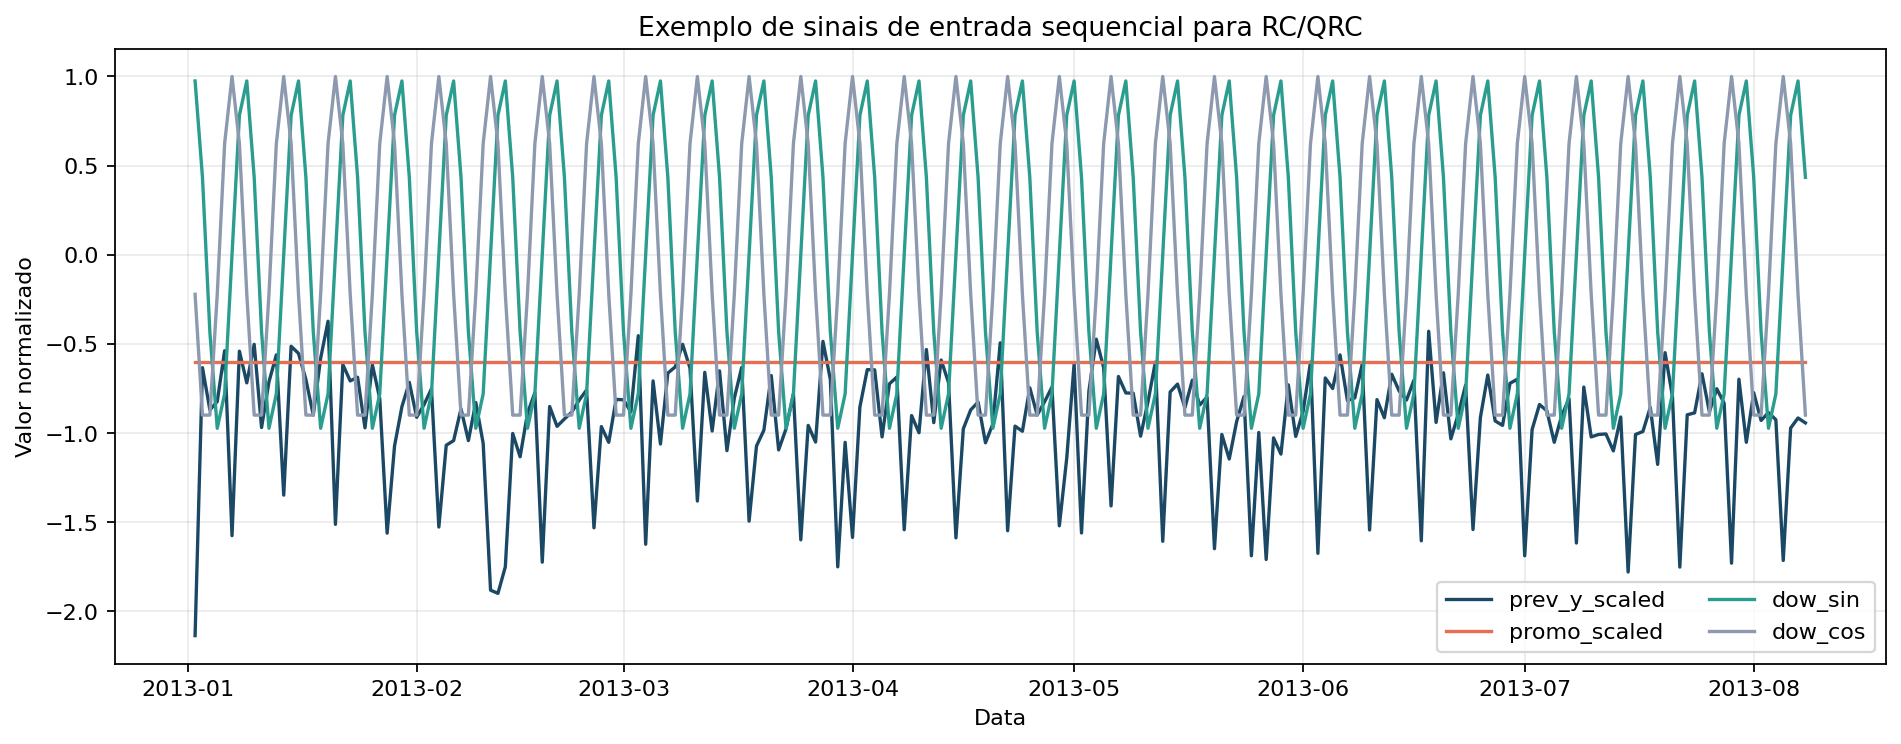
\includegraphics[width=\linewidth,keepaspectratio]{computational_results_20260407_000554/sequential_inputs_example.png}
\caption{Exemplo dos sinais de entrada sequenciais usados pelo RC.}
\end{figure}

A imagem de entrada sequencial mostra que o reservatório não recebe apenas uma série de vendas crua. Ele recebe uma codificacao temporal e exógena compacta.

\begin{figure}[htbp]
\centering
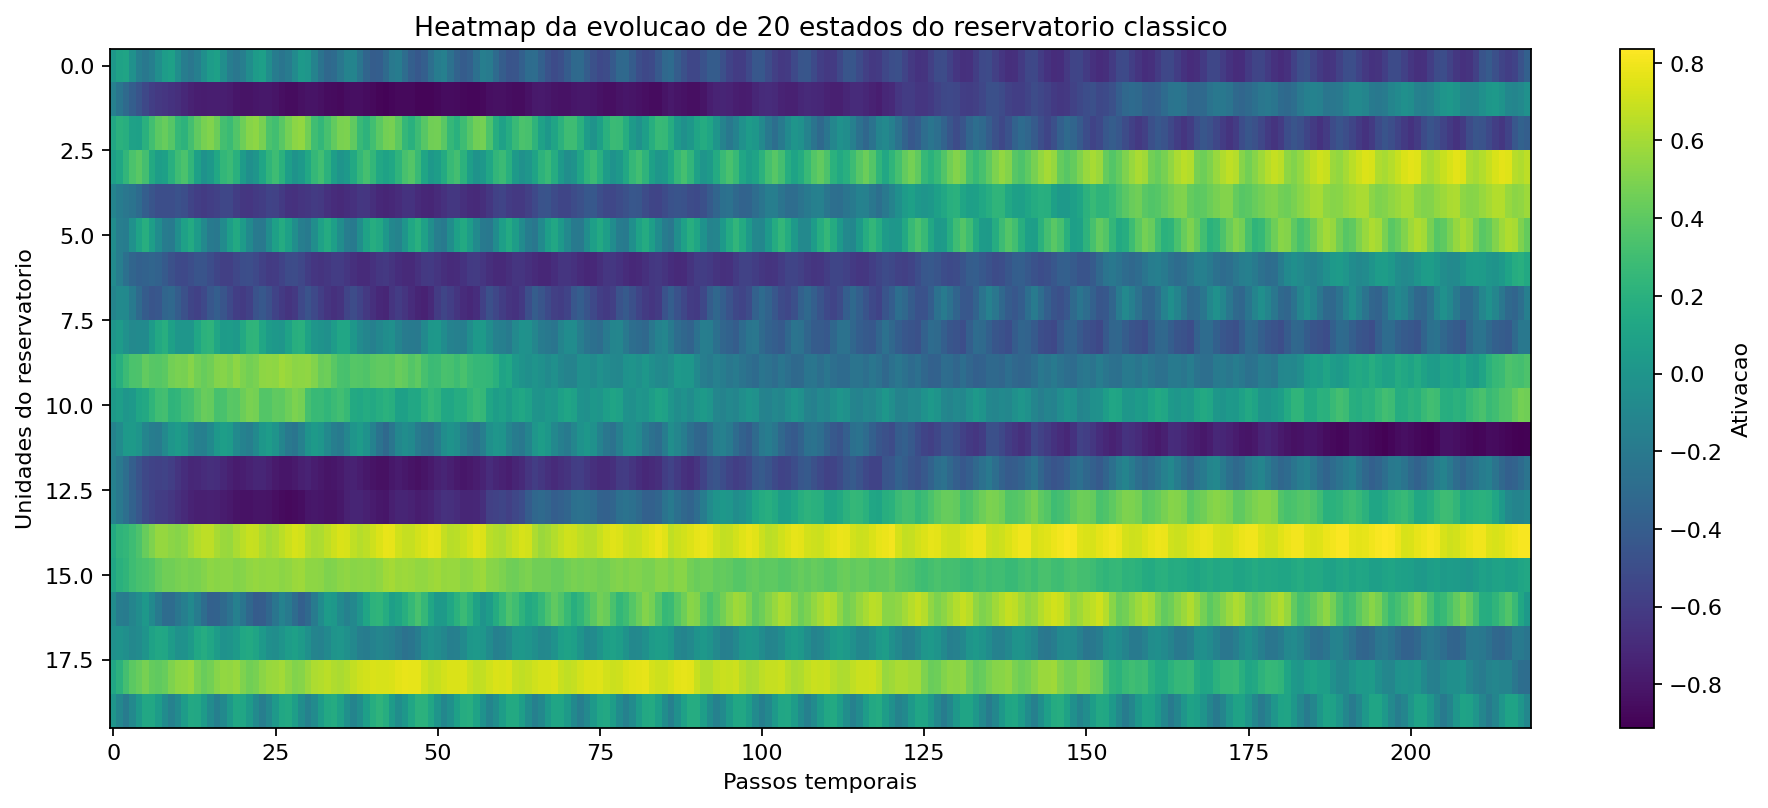
\includegraphics[width=\linewidth,keepaspectratio]{computational_results_20260407_000554/rc_state_heatmap.png}
\caption{Heatmap dos estados internos do reservatório clássico no recorte adotado no Favorita.}
\end{figure}

O heatmap dos estados ilustra duas ideias importantes:

\begin{enumerate}
\def\labelenumi{\arabic{enumi}.}
\tightlist
\item
  unidades diferentes respondem de modos diferentes ao mesmo estimulo;
\item
  a memória do reservatório não é um único lag explícito, mas uma combinacao distribuída de estados.
\end{enumerate}

Em outras palavras, RC constroi uma base dinâmica de features sem precisar enumerar manualmente toda a interação temporal. Isso sustenta bem a \textbf{qualidade conceitual da representação interna}, mas ainda não diz, por si só, se a previsão final e forte.

\section{Como avaliar a qualidade do RC sem misturar conceitos}\label{9-como-avaliar-a-qualidade-do-rc-sem-misturar-conceitos}

A avaliação do RC fica mais clara quando separamos três perguntas que muitas vezes sao misturadas.

\begin{longtable}[]{@{}lll@{}}
\toprule\noalign{}
Eixo de avaliação & Pergunta correta & Evidencia usada neste artigo \\
\midrule\noalign{}
\endhead
\bottomrule\noalign{}
\endlastfoot
Representação interna & Os estados reagem de forma heterogenea, não linear e com memória distribuída? & \texttt{sequential\_inputs\_example.png} e \texttt{rc\_state\_heatmap.png} \\
Previsão final & O readout produz erro baixo no mesmo split e contra baselines honestos? & \texttt{rc\_quality\_preview.csv} \\
Estabilidade experimental & O resultado se sustenta quando seed e hiperparâmetros mudam? & \texttt{rc\_seed\_stability\_summary.csv} e \texttt{rc\_washout\_sweep.csv} \\
\end{longtable}

Essa separacao evita um erro comum: tratar um heatmap interessante como prova suficiente de que a saida prevista e boa. Um estado interno pode ser didaticamente convincente e, ainda assim, produzir uma previsão final medíocre se o readout receber uma dinâmica mal configurada.

\section{Primeira evidencia quantitativa da saida do RC}\label{10-primeira-evidencia-quantitativa-da-saida-do-rc}

A tabela abaixo posiciona o RC default contra duas referencias honestas no mesmo bloco de teste de \texttt{90} dias.

\begin{longtable}[]{@{}llllll@{}}
\toprule\noalign{}
Modelo & Janela & MAE & RMSE & WAPE & sMAPE \\
\midrule\noalign{}
\endhead
\bottomrule\noalign{}
\endlastfoot
ETS & teste (90 dias) & 216.303 & 307.638 & 0.0999 & 0.1042 \\
Seasonal Naive & teste (90 dias) & 259.067 & 352.280 & 0.1196 & 0.1361 \\
RC default & teste (90 dias) & 324.294 & 423.417 & 0.1498 & 0.1653 \\
\end{longtable}

Duas leituras importam aqui:

\begin{enumerate}
\def\labelenumi{\arabic{enumi}.}
\tightlist
\item
  o RC default funciona de ponta a ponta: ele gera previsões finitas, mede erro e pode ser comparado sob o mesmo protocolo temporal;
\item
  isso ainda não basta para chama-lo de melhor solucao neste recorte: seu \texttt{MAE} ficou 25.2\% acima do \texttt{Seasonal\ Naive} e 49.9\% acima do \texttt{ETS}.
\end{enumerate}

Esse ponto é central para a honestidade científica do texto. O artigo agora não apenas explica \textbf{como} o RC funciona; ele também mostra \textbf{o que a configuração default entrega} quando confrontada com baselines sérios.

\section{Estabilidade experimental: a seed também faz parte da historia}\label{11-estabilidade-experimental-a-seed-tambuxe9m-faz-parte-da-historia}

Um único run pode dar uma impressao excessivamente otimista ou pessimista sobre RC. Por isso, executamos dez seeds para três configurações simples.

\begin{longtable}[]{@{}llllll@{}}
\toprule\noalign{}
Configuração & Seeds & MAE & RMSE & WAPE & sMAPE \\
\midrule\noalign{}
\endhead
\bottomrule\noalign{}
\endlastfoot
default & 10 & 565.337 +/- 504.007 & 686.563 +/- 570.807 & 0.2611 +/- 0.2327 & 0.2557 +/- 0.1505 \\
sr = 0.20 & 10 & 477.982 +/- 285.463 & 604.875 +/- 373.503 & 0.2207 +/- 0.1318 & 0.2269 +/- 0.1016 \\
sr = 0.20, leak = 0.30 & 10 & 453.504 +/- 230.676 & 576.555 +/- 325.866 & 0.2094 +/- 0.1065 & 0.2185 +/- 0.0817 \\
\end{longtable}

Três fatos se destacam:

\begin{enumerate}
\def\labelenumi{\arabic{enumi}.}
\tightlist
\item
  a configuração default apresentou alta variabilidade: \texttt{MAE} médio de 565.337 com desvio-padrão de 504.007;
\item
  no default, a faixa observada foi larga: de 275.064 até 1966.124;
\item
  um ajuste simples para \texttt{spectral\_radius\ =\ 0.20} e \texttt{leak\_rate\ =\ 0.30} reduziu o \texttt{MAE} médio em 19.8\% e o desvio-padrão em 54.2\% em relação ao default.
\end{enumerate}

Esse resultado não invalida o RC. Ele mostra algo mais útil: o desempenho do reservatório depende do regime dinamico em que ele opera. Em outras palavras, \texttt{seed} e hiperparâmetros fazem parte da qualidade experimental do modelo.

\section{O que o washout realmente controla}\label{12-o-que-o-washout-realmente-controla}

O \texttt{washout} decide quantos passos iniciais sao descartados antes de o readout ver os estados internos. Conceitualmente, ele separa transiente de inicialização de dinâmica útil. Experimentalmente, ele muda o erro.

\begin{longtable}[]{@{}lllll@{}}
\toprule\noalign{}
Washout & MAE & RMSE & WAPE & sMAPE \\
\midrule\noalign{}
\endhead
\bottomrule\noalign{}
\endlastfoot
0 & 325.718 & 411.319 & 0.1504 & 0.1651 \\
7 & 317.567 & 402.268 & 0.1466 & 0.1613 \\
14 & 324.294 & 423.417 & 0.1498 & 0.1653 \\
21 & 327.744 & 434.786 & 0.1513 & 0.1677 \\
28 & 334.848 & 446.066 & 0.1546 & 0.1722 \\
42 & 330.511 & 439.718 & 0.1526 & 0.1695 \\
\end{longtable}

Neste recorte, \texttt{washout\ =\ 7} foi o melhor valor entre os testados, com \texttt{MAE\ =\ 317.567}. A licao pratica e simples:

\begin{itemize}
\tightlist
\item
  \texttt{washout} muito curto pode contaminar o readout com estados ainda dominados pela inicialização;
\item
  \texttt{washout} excessivo desperdica observações úteis de treino.
\end{itemize}

\section{Como escolher os hiperparâmetros centrais sem adivinhar}\label{13-como-escolher-os-hiperparuxe2metros-centrais-sem-adivinhar}

O leitor não precisa decorar uma grade enorme de tuning para começar. O mais importante e entender o papel de cada hiperparâmetro e que tipo de comportamento esperar quando ele varia.

\begin{longtable}[]{@{}llll@{}}
\toprule\noalign{}
Hiperparâmetro & Papel & Faixa inicial pratica & Evidencia no recorte \\
\midrule\noalign{}
\endhead
\bottomrule\noalign{}
\endlastfoot
\texttt{spectral\_radius} & controla persistencia e regime dinamico do reservatório & \texttt{0.20} a \texttt{0.60} & \texttt{0.20} gerou MAE 275.280; \texttt{0.80} degradou para 871.792. O default \texttt{0.60} ficou em 324.294. \\
\texttt{leak\_rate} & controla a velocidade de atualizacao do estado & \texttt{0.10} a \texttt{0.30} & \texttt{0.30} foi melhor que o default \texttt{0.15} (317.767 vs. 324.294); \texttt{0.50} colapsou para 770.680. \\
\texttt{washout} & remove o transiente de inicialização antes do treino do readout & \texttt{7} a \texttt{21} & Nesta série, o melhor valor testado foi \texttt{7} com MAE 317.567; acima de \texttt{28} o erro voltou a subir. \\
\texttt{n\_reservoir} & define a capacidade representacional do estado interno & \texttt{80} como ponto de partida, com vizinhança \texttt{40} a \texttt{120} & \texttt{80} foi o melhor ponto entre os testados (324.294); \texttt{40} subiu para 1278.623 e \texttt{160} para 430.945. \\
\end{longtable}

O ponto didático aqui e decisivo: \texttt{spectral\_radius}, \texttt{leak\_rate}, \texttt{washout} e \texttt{n\_reservoir} não sao botoes arbitrarios. Eles controlam memória, velocidade de resposta, uso do transiente e capacidade representacional.

\section{O que este artigo já prova, e o que ainda deixa em aberto}\label{14-o-que-este-artigo-juxe1-prova-e-o-que-ainda-deixa-em-aberto}

\subsection{O que já esta claro}\label{141-o-que-juxe1-esta-claro}

\begin{itemize}
\tightlist
\item
  a representação interna do RC e boa como mecanismo conceitual: os estados sao heterogeneos, não lineares e coerentes com a ideia de memória distribuída;
\item
  a previsão final do RC e mensuravel e comparavel; portanto, o artigo já não depende apenas de intuição;
\item
  a estabilidade experimental precisa ser reportada de forma explícita, porque a variação por seed e relevante.
\end{itemize}

\subsection{O que ainda não esta encerrado}\label{142-o-que-ainda-nuxe3o-esta-encerrado}

\begin{itemize}
\tightlist
\item
  este artigo ainda não fecha o benchmark completo da série;
\item
  ele não substitui uma comparação ampla com \texttt{Prophet}, \texttt{XGBoost}, \texttt{LSTM} e \texttt{QRC};
\item
  ele não pretende vender o RC como melhor modelo neste recorte, e sim estabelecer uma base correta para julga-lo.
\end{itemize}

Essa delimitacao melhora o artigo, porque troca promessa vaga por evidencia observável.

\section{Passo-a-passo para estudar ou modificar o RC do projeto}\label{15-passo-a-passo-para-estudar-ou-modificar-o-rc-do-projeto}

Um leitor que queira estudar a implementação deve seguir esta ordem:

\begin{enumerate}
\def\labelenumi{\arabic{enumi}.}
\tightlist
\item
  abrir \texttt{code/common/sequential\_features.py};
\item
  verificar como o vetor \texttt{u\_t} e construído;
\item
  abrir \texttt{code/rc/model.py} e localizar \texttt{RCConfig};
\item
  ler \texttt{EchoStateReservoir.step()} junto da equação do artigo;
\item
  ler \texttt{fit\_rc\_readout()} e localizar o \texttt{washout};
\item
  executar \texttt{python\ code/rc/run.py};
\item
  validar o comportamento com \texttt{pytest\ code/rc/test\_model.py}.
\end{enumerate}

Essa ordem importa. Se o leitor abrir apenas \texttt{run.py}, perde a correspondencia entre teoria e implementação.

\section{Conclusão}\label{16-conclusuxe3o}

RC agora esta formulado no contexto do projeto com um nível maior de rigor. O artigo continua didático, mas deixa de depender apenas de intuição: ele mostra como o estado interno evolui, como a previsão sai do readout e como medir, de forma honesta, se essa saida e boa e estável. A resposta correta para este recorte e clara: a representação interna do RC e forte como objeto conceitual; a previsão final default e promissora, mas ainda inferior a baselines clássicos fortes; e a estabilidade experimental exige cuidado com seed e hiperparâmetros. Isso prepara melhor o leitor para os artigos seguintes, porque o próximo passo deixa de ser "confiar no RC" e passa a ser "testar o RC com método".

\section*{Entregaveis associados no repositorio}\label{entregaveis-associados-no-repositorio}

\begin{itemize}
\tightlist
\item
  implementação do RC: \texttt{code/rc/model.py}
\item
  execucao do RC: \texttt{code/rc/run.py}
\item
  testes do RC: \texttt{code/rc/test\_model.py}
\item
  construcao de entrada sequencial: \texttt{code/common/sequential\_features.py}
\item
  leitura quantitativa inicial: \texttt{computational\_results\_20260407\_000554/rc\_quality\_preview.csv}
\item
  estabilidade em múltiplas seeds: \texttt{computational\_results\_20260407\_000554/rc\_seed\_stability\_summary.csv}
\item
  sweep de \texttt{washout}: \texttt{computational\_results\_20260407\_000554/rc\_washout\_sweep.csv}
\item
  artefatos deste artigo: \texttt{computational\_results\_20260407\_000554/}
\end{itemize}

\section{Referências}\label{referencias}

\begin{thebibliography}{9}

\bibitem{jaeger2001}
JAEGER, H. \textbf{The ``echo state'' approach to analysing and training recurrent neural networks}. Bonn: German National Research Center for Information Technology (GMD), 2001.

\bibitem{lukosevicius2009}
LUKOSEVICIUS, M.; JAEGER, H. \textbf{Reservoir computing approaches to recurrent neural network training}. \emph{Computer Science Review}, v. 3, n. 3, p. 127--149, 2009.

\bibitem{lukosevicius2012}
LUKOSEVICIUS, M. \textbf{A practical guide to applying echo state networks}. In: MONTAVON, G.; ORR, G. B.; MÜLLER, K.-R. (org.). \emph{Neural Networks: Tricks of the Trade}. 2. ed. Berlin: Springer, 2012. p. 659--686.

\bibitem{fujii2017}
FUJII, K.; NAKAJIMA, K. \textbf{Harnessing disordered-ensemble quantum dynamics for machine learning}. \emph{Physical Review Applied}, v. 8, n. 2, 024030, 2017.

\end{thebibliography}

            \end{document}
